\section{Balance Controller (Task 2)}
\label{sec:balance}

\subsection{Plant Transfer Function}
With the redesigned inner wheel-speed loop of Task~\ref{sec:wheel-speed} closed, the plant seen by the balance controller is identified by linearising the Simulink model from the velocity reference \texttt{/vel\_ref} to the tilt-angle output (port~1 of the \texttt{/robot with balance} subsystem). The resulting transfer function $G_{tilt}(s)$ is seventh order and open-loop unstable, with one pole in the right-half plane near $+8.89\,\mathrm{rad/s}$ corresponding to the inverted-pendulum falling mode. Relinearising against the Day~5 on-floor inner loop (Section~\ref{sec:wheel-speed}) also shifts the peak of $|G_{tilt}|$ from $5.95$ to $8.03\,\mathrm{rad/s}$ --- the faster inner loop changes the frequency at which the tilt-to-velocity plant has its strongest response, which in turn moves the post-integrator below.

\begin{figure}[H]
    \centering
    \begin{subfigure}[t]{0.48\linewidth}
        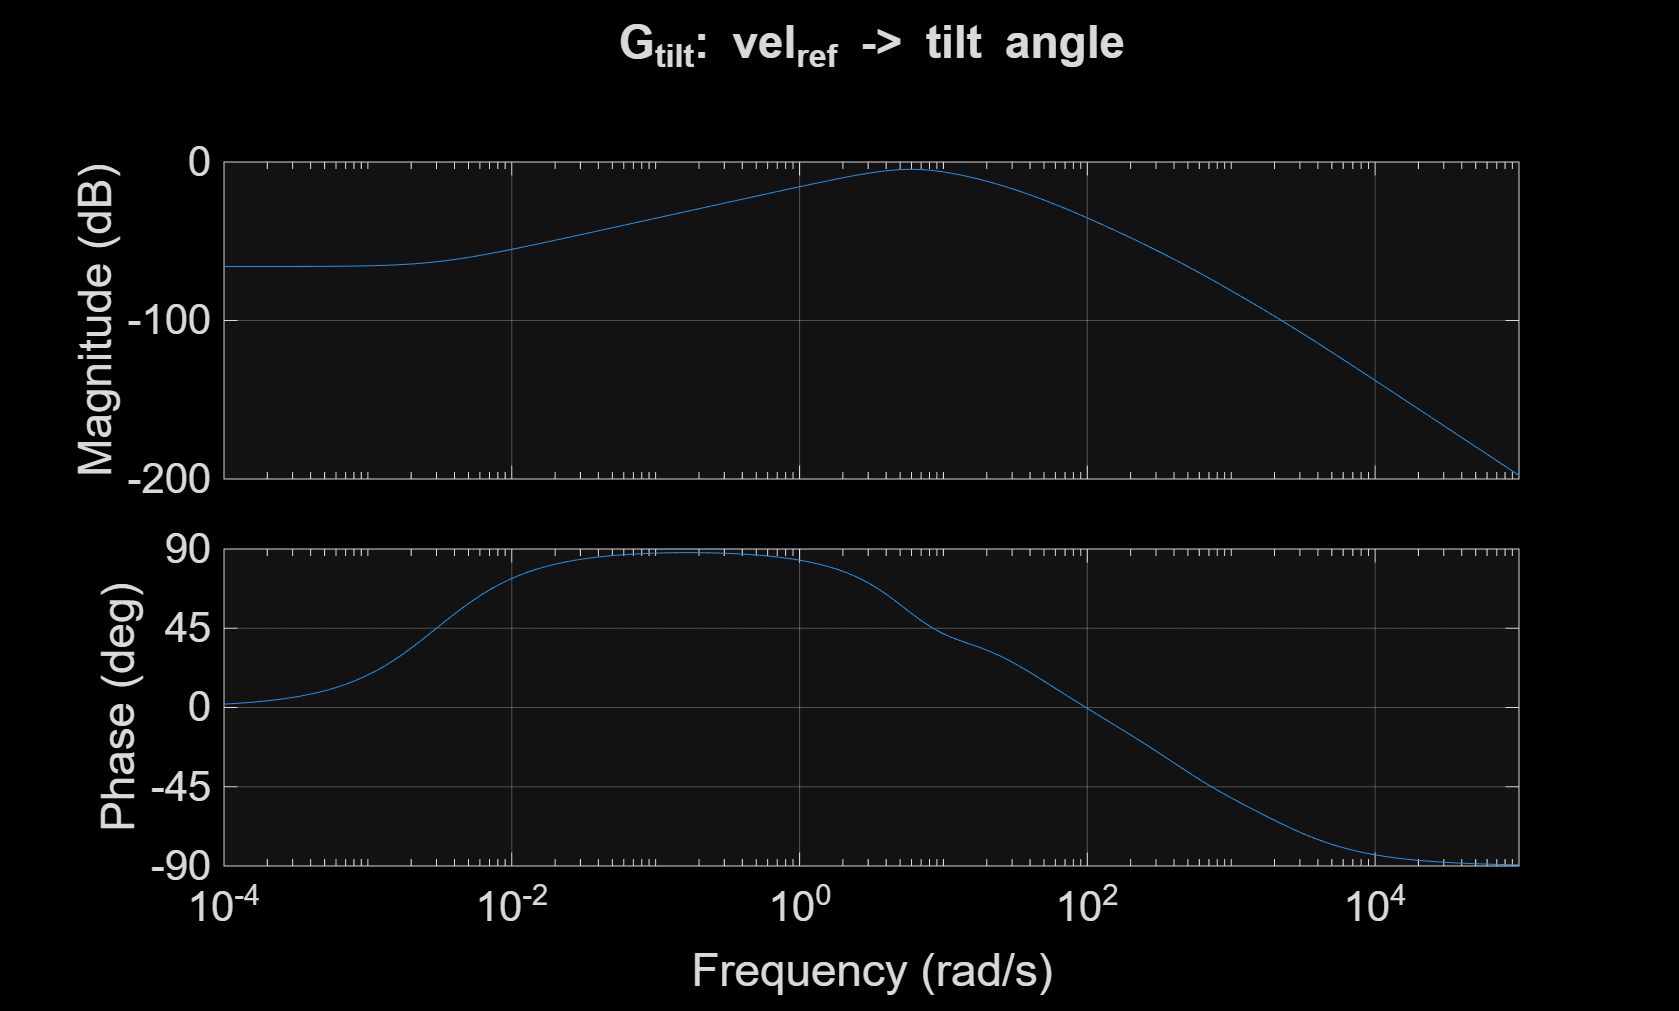
\includegraphics[width=\linewidth]{images/regbot_Gtilt_bode.png}
        \caption{Bode plot of $G_{tilt}$.}
        \label{fig:gtilt_bode}
    \end{subfigure}
    \hfill
    \begin{subfigure}[t]{0.48\linewidth}
        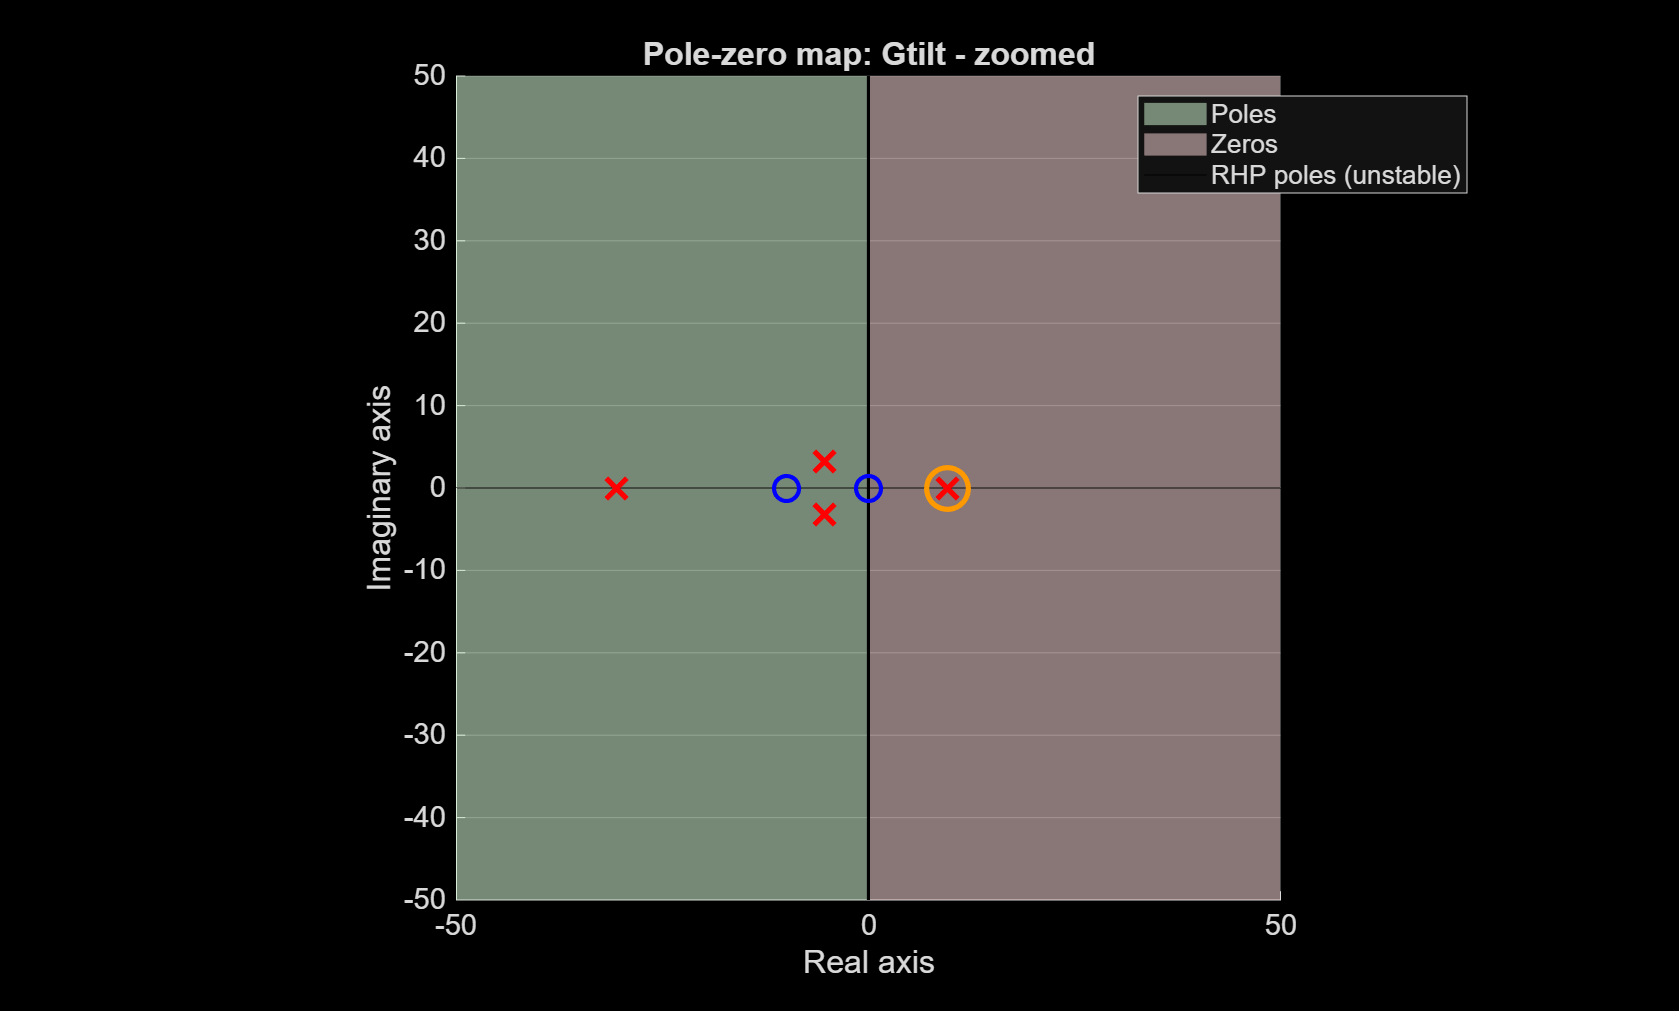
\includegraphics[width=\linewidth]{images/regbot_Gtilt_pzmap_zoom.png}
        \caption{Pole-zero map (zoom). The orange ring marks the single RHP pole.}
        \label{fig:gtilt_pz}
    \end{subfigure}
    \caption{Plant from velocity reference to tilt angle, $G_{tilt}(s)$.}
\end{figure}

\subsection{Controller Design — Lecture 10 Method 2}
We follow Method~2 from Lecture~10: (i) decide $\mathrm{sign}(K_{PS})$ from a Nyquist check, (ii) add a post-integrator to shape $|G|$ into a monotonically decreasing form, (iii) design an outer PI-Lead on the stabilised plant, (iv) verify the closed loop.

\paragraph{Step 1 — Nyquist sign check.}
$G_{tilt}$ has positive DC gain ($+5.04\cdot10^{-4}\,\mathrm{rad/(m/s)}$) and $P = 1$ right-half-plane pole. The Nyquist criterion requires $N = -P = -1$ (one counter-clockwise encirclement of $(-1,0)$), which a positive $K_{PS}$ cannot provide. We therefore set $\mathrm{sign}(K_{PS}) = -1$ and absorb the minus sign into the post-integrator.

\paragraph{Step 2 — Post-integrator.}
Locate the peak of $|G_{tilt}|$ on the Bode magnitude curve and place the PI zero there. With the redesigned inner loop in place the peak moves up:
\begin{equation}
    |G_{tilt}|_{\max} = 0.413 \quad \text{at} \quad \omega_{\mathrm{peak}} = 8.03\,\mathrm{rad/s}
    \;\Longrightarrow\;
    \tau_{i,\mathrm{post}} = \frac{1}{\omega_{\mathrm{peak}}} = 0.1245\,\mathrm{s}.
\end{equation}
The stabilised plant used for outer-loop design is
\begin{equation}
    G_{tilt,\mathrm{post}}(s)
    = -\,C_{PI,\mathrm{post}}(s)\,G_{tilt}(s),
    \qquad
    C_{PI,\mathrm{post}}(s) = \frac{\tau_{i,\mathrm{post}}\,s + 1}{\tau_{i,\mathrm{post}}\,s}.
\end{equation}

\begin{figure}[H]
    \centering
    \begin{subfigure}[t]{0.48\linewidth}
        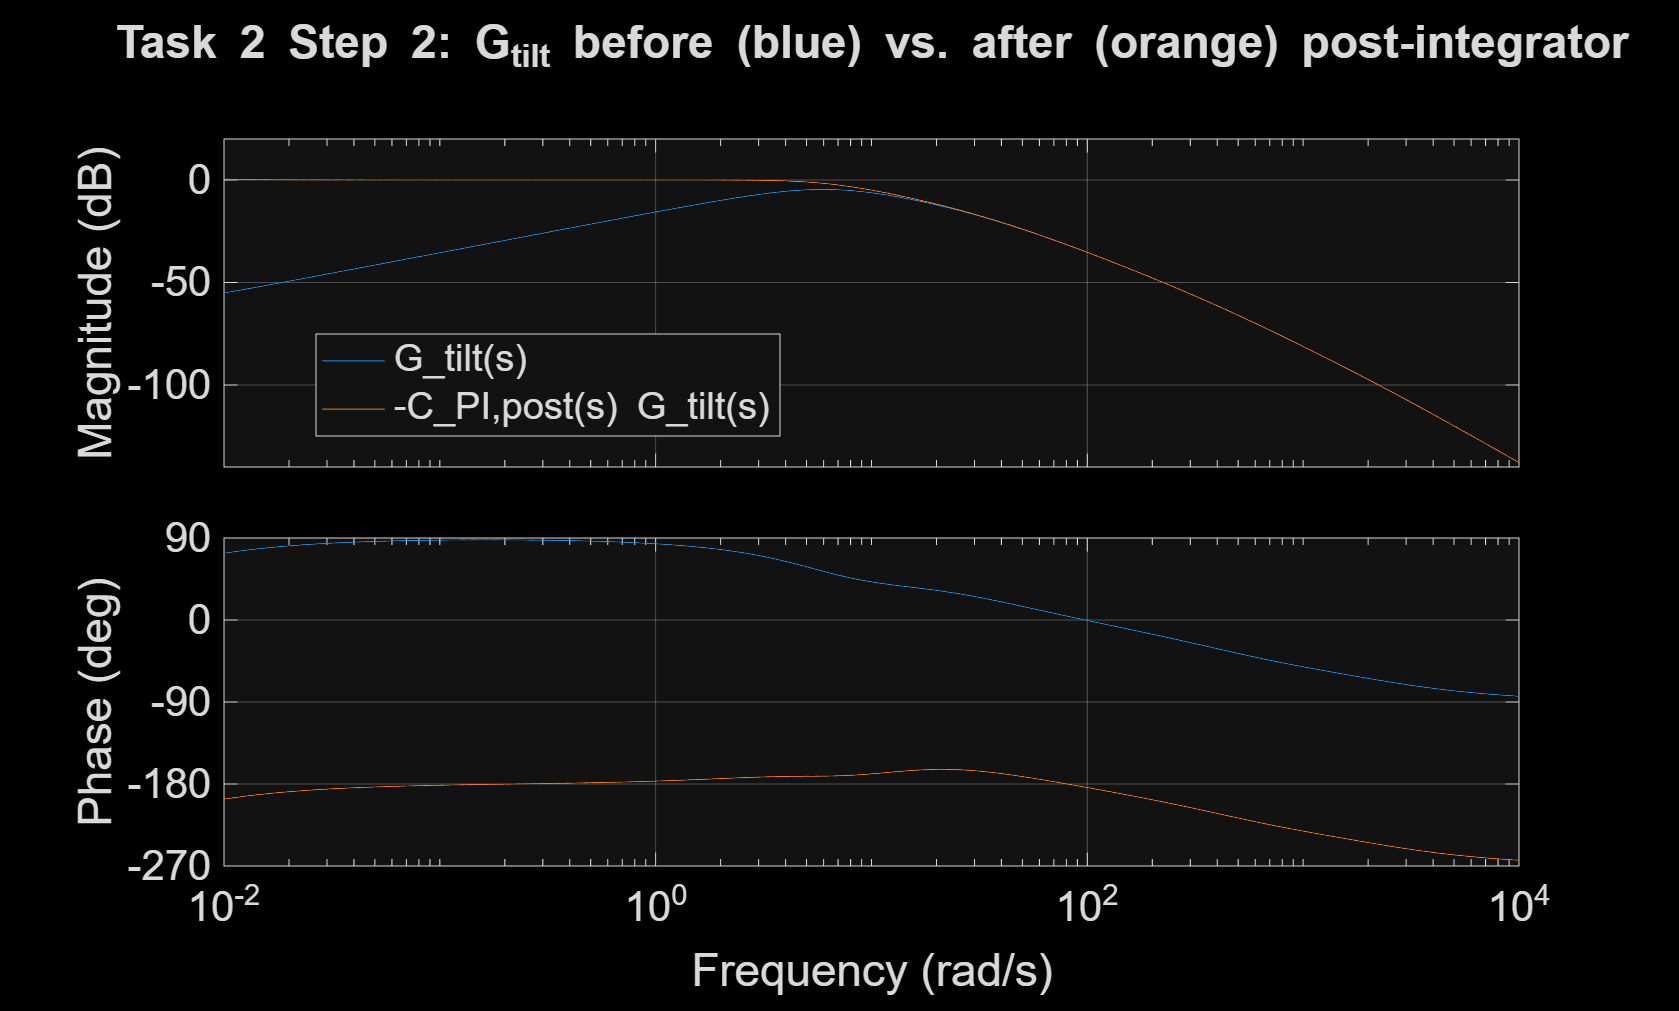
\includegraphics[width=\linewidth]{images/regbot_task2_bode_post.png}
        \caption{$G_{tilt}$ (blue) vs.\ $G_{tilt,\mathrm{post}}$ (orange). After the post-integrator the magnitude is monotonically decreasing beyond $\omega_{\mathrm{peak}}$.}
    \end{subfigure}
    \hfill
    \begin{subfigure}[t]{0.48\linewidth}
        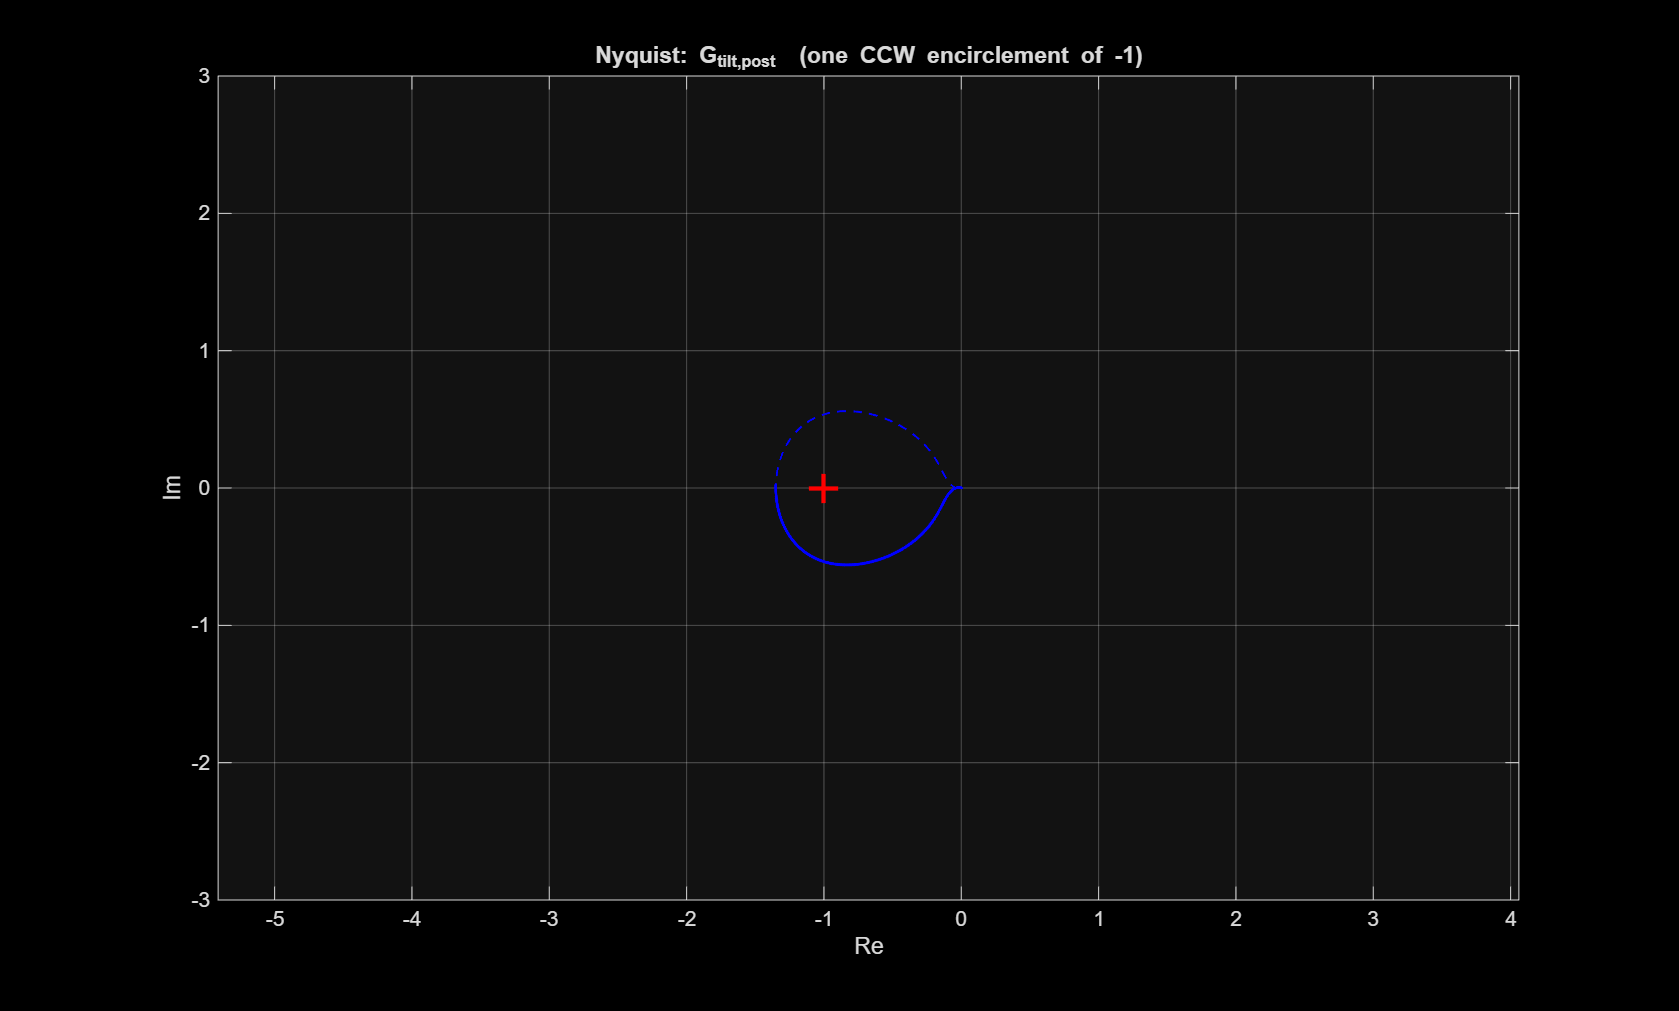
\includegraphics[width=\linewidth]{images/regbot_task2_nyquist_post.png}
        \caption{Nyquist of $G_{tilt,\mathrm{post}}$. One CCW encirclement of $(-1,0)$, matching $P = 1$.}
    \end{subfigure}
    \caption{Stabilisation via the post-integrator (Method~2 Step~2).}
\end{figure}

\paragraph{Step 3 — Outer PI-Lead on $G_{tilt,\mathrm{post}}$.}
Specifications: $\omega_c = 15\,\mathrm{rad/s}$, $\gamma_M = 60^{\circ}$, $N_i = 3$.

The PI zero is placed at $\omega_c/N_i$:
\begin{equation}
    \tau_i = \frac{N_i}{\omega_c} = 0.200\,\mathrm{s},
    \qquad
    C_{PI}(s) = \frac{\tau_i\,s + 1}{\tau_i\,s}.
\end{equation}

Phase balance at $\omega_c$:
\begin{equation}
    \phi_{\mathrm{Lead}}
    = -180^{\circ} + \gamma_M - \angle G_{tilt,\mathrm{post}}(j\omega_c) - \angle C_{PI}(j\omega_c),
\end{equation}
with the numerical values from the redesigned post-integrated plant
\begin{align*}
    \angle G_{tilt,\mathrm{post}}(j\omega_c) &= -135.09^{\circ}, \\
    \angle C_{PI}(j\omega_c) = -\arctan(1/N_i) &= -18.43^{\circ}, \\
    \phi_{\mathrm{Lead}} &= +33.52^{\circ}.
\end{align*}
The required Lead is noticeably smaller than it would be without the redesigned inner loop ($+63.8^{\circ}$ on the Day~4 design). The post-integrated plant has more available phase at crossover because its magnitude peak has moved nearer $\omega_c$, so less phase lift is needed from the Lead.

The Lead is realised through the gyro measurement $\dot\theta = s\theta$, avoiding the filter pole of a proper Lead:
\begin{equation}
    (\tau_d\,s + 1)\,\theta = \tau_d\,\dot\theta + \theta,
    \qquad
    \tau_d = \frac{\tan\phi_{\mathrm{Lead}}}{\omega_c} = \frac{\tan 33.52^{\circ}}{15} = 0.0442\,\mathrm{s}.
\end{equation}
This is $67\,\%$ smaller than the value the original Day~4-based design produced ($0.1355\,\mathrm{s}$). Physically, the inner loop is now fast enough that the balance controller does not have to lean as heavily on the Lead to restore phase at $\omega_c$.

The loop gain is chosen from $|L(j\omega_c)| = 1$:
\begin{equation}
    \bigl|C_{PI}(j\omega_c)\,C_{\mathrm{Lead}}(j\omega_c)\,G_{tilt,\mathrm{post}}(j\omega_c)\bigr| = 0.833,
    \qquad
    K_P = \frac{1}{0.833} = 1.1999.
\end{equation}

Gathering the four blocks, the full controller from pitch measurement to $v_{\mathrm{ref}}$ is
\begin{equation}
    C_\mathrm{total}(s)
    = K_P\cdot
      \underbrace{\frac{-(\tau_{i,\mathrm{post}}s + 1)}{\tau_{i,\mathrm{post}}s}}_{\text{sign + post-integrator}}\cdot
      \underbrace{\frac{\tau_i s + 1}{\tau_i s}}_{\text{outer PI}}\cdot
      \underbrace{(\tau_d s + 1)}_{\text{Lead (gyro)}}.
\end{equation}

\paragraph{Step 4 — Closed-loop verification.}
From \texttt{margin(L\_tilt)}: achieved $\omega_c = 15.00\,\mathrm{rad/s}$, $\gamma_M = 60.00^{\circ}$, $GM = -5.58\,\mathrm{dB}$. A negative gain margin is expected here: for plants with $P = 1$ the gain margin reported by \texttt{margin} is a \emph{lower} bound on $|K|$ rather than an upper bound. All closed-loop poles lie in the left half plane. A linear-model initial-condition test (impulse on pitch, closed pitch loop) settles in $1.34\,\mathrm{s}$, down from $1.55\,\mathrm{s}$ before the inner-loop redesign --- the outer balance loop regulates disturbances slightly faster when the inner loop is properly fast.

\begin{table}[H]
    \centering
    \caption{Final design parameters for Task~2.}
    \begin{tabular}{@{}lll@{}}
        \toprule
        Parameter & Symbol & Value \\
        \midrule
        Target crossover          & $\omega_c$            & $15\,\mathrm{rad/s}$ \\
        Target phase margin       & $\gamma_M$            & $60^{\circ}$ \\
        PI zero ratio             & $N_i$                 & $3$ \\
        Post-integrator           & $\tau_{i,\mathrm{post}}$ & $0.1245\,\mathrm{s}$ \\
        Outer PI                  & $\tau_i$              & $0.2000\,\mathrm{s}$ \\
        Lead (gyro)               & $\tau_d$              & $0.0442\,\mathrm{s}$ \\
        Loop gain                 & $K_P$                 & $1.1999$ \\
        \bottomrule
    \end{tabular}
\end{table}

\subsection{Bode Plot (Open-Loop)}
\begin{figure}[H]
    \centering
    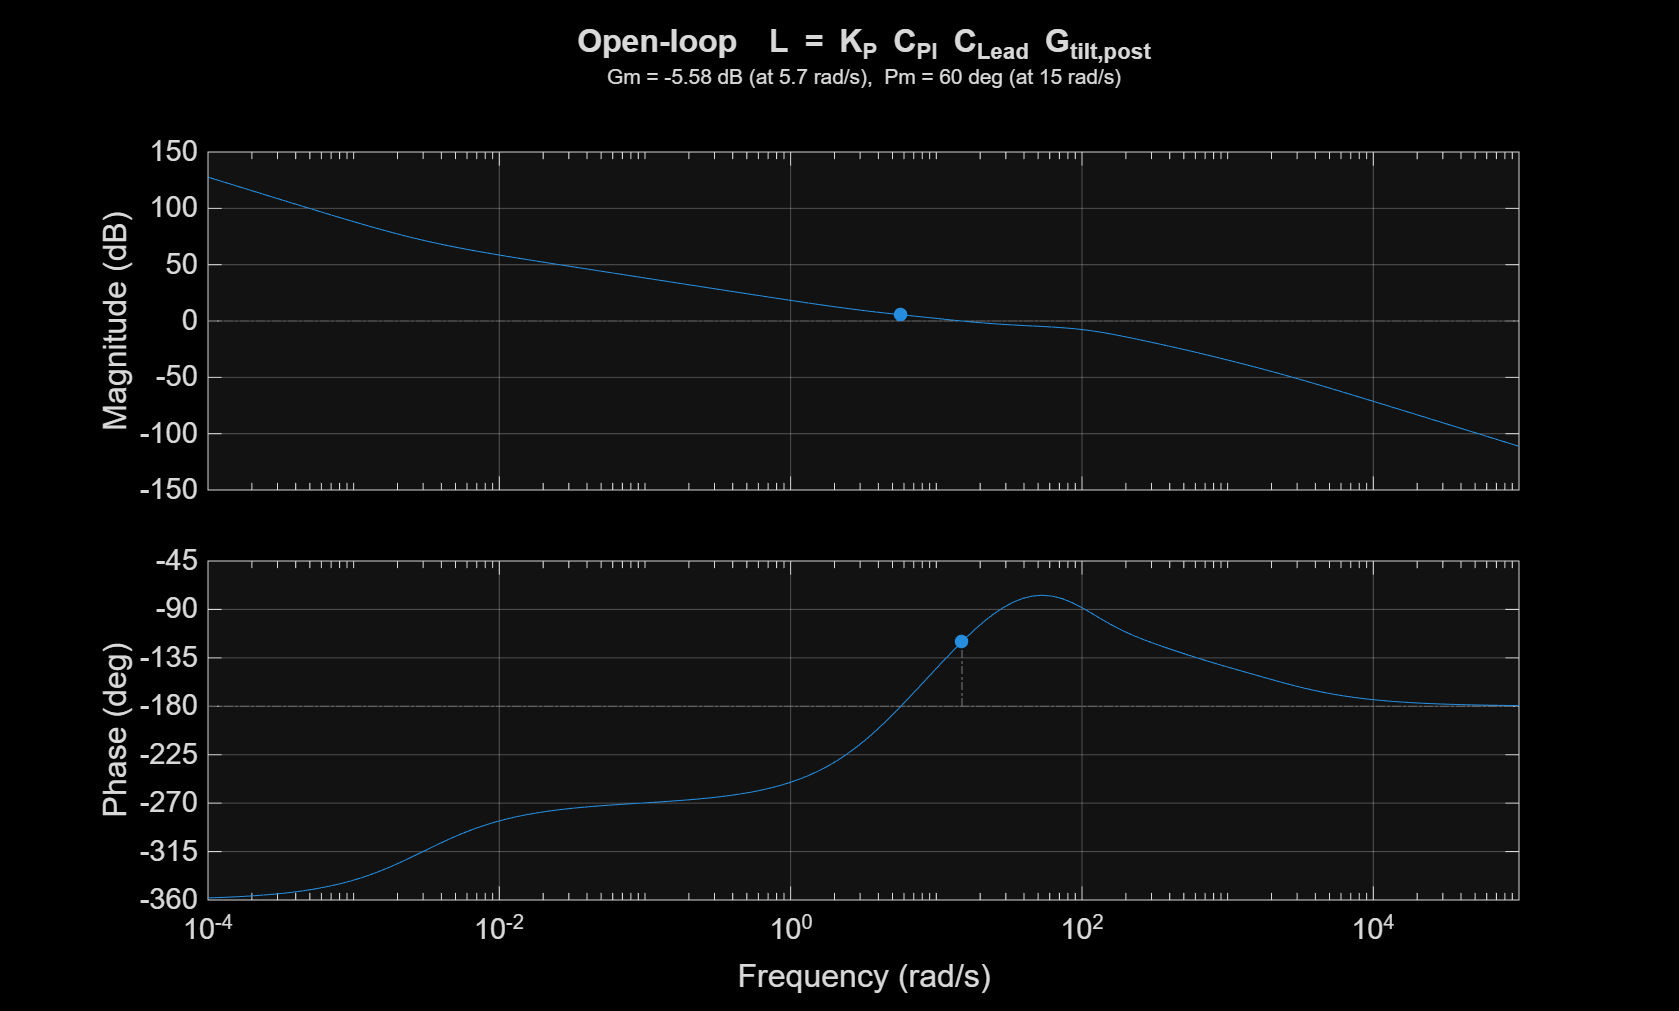
\includegraphics[width=0.7\linewidth]{images/regbot_task2_loop_bode.png}
    \caption{Open-loop Bode of $L(s) = K_P\,C_{PI}(s)\,C_{\mathrm{Lead}}(s)\,G_{tilt,\mathrm{post}}(s)$. Crossover at $\omega_c = 15\,\mathrm{rad/s}$ with $\gamma_M = 60^{\circ}$.}
    \label{fig:task2_loop_bode}
\end{figure}

\subsection{Simulation Results}
The balance controller is wired in Simulink so that the gyro-based Lead is combined with pitch \emph{before} the error sum (multiplicative Lead in series). Two simulation tests validate the design:

\paragraph{Initial-condition recovery.} With $\theta_0 = 10^{\circ}$ initial tilt and no external push, the full non-linear model drives pitch from $0.175\,\mathrm{rad}$ to zero within roughly $0.3\,\mathrm{s}$ and settles completely by $t \approx 2\,\mathrm{s}$. Peak motor voltage is $2.8\,\mathrm{V}$, well inside the $\pm 9\,\mathrm{V}$ saturation limit (Figure~\ref{fig:task2_sim_recovery}).

\begin{figure}[H]
    \centering
    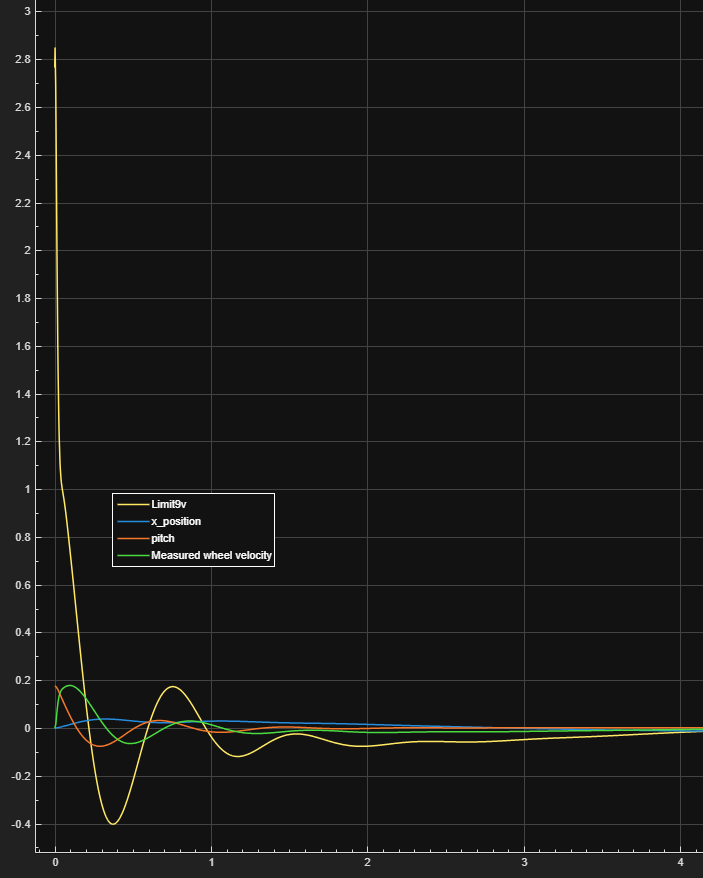
\includegraphics[width=0.8\linewidth]{images/regbot_task2_sim_recovery_10deg_v3.png}
    \caption{Simulink recovery from $\theta_0 = 10^{\circ}$ with the Day 5 on-floor design. Yellow: pitch in radians ($0.175\,\mathrm{rad} \to 0$ within $\approx 0.3\,\mathrm{s}$). Blue: motor voltage (peak $\approx 2.8\,\mathrm{V}$, no saturation).}
    \label{fig:task2_sim_recovery}
\end{figure}

\paragraph{Push-disturbance rejection.} A 1\,N, 0.1\,s push applied at the top of the robot at $t = 1$\,s is rejected within $\approx 2$\,s with two decaying cycles, no voltage saturation, and a small residual position offset (Figure~\ref{fig:task2_sim_push}). The residual $x$-offset is expected: Task~2 closes only the balance and velocity loops; the position loop is added in Task~4.

\begin{figure}[H]
    \centering
    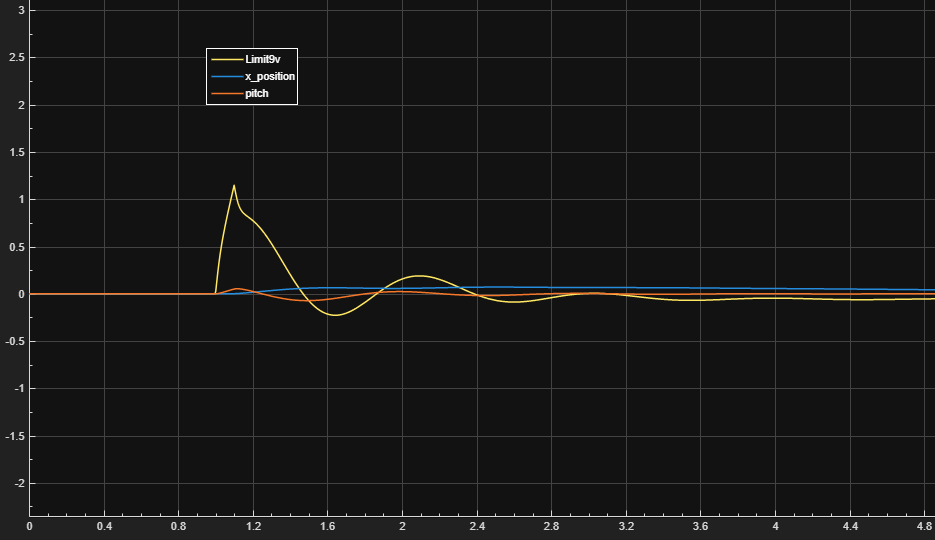
\includegraphics[width=0.85\linewidth]{images/regbot_task2_sim_push.png}
    \caption{Regulation response to a 1\,N / 0.1\,s push at $t = 1$\,s (Day 4 controller; retained for the qualitative push illustration). Yellow: motor voltage. Blue: wheel position. Red: pitch. Tilt recovers within $\approx 2$\,s, motor voltage stays well inside the limit, wheel position settles at a small residual offset.}
    \label{fig:task2_sim_push}
\end{figure}

\subsection{REGBOT Experiment}
\label{sec:task2_hw}
Task~2 was validated on the physical robot with Test~3a (\texttt{vel=0, bal=1, log=15 : time=10}). The robot was held upright near the balance point, the mission was started, and the robot was released gently. Balance had to be maintained for 10\,s with drift no larger than $0.5\,\mathrm{m}$.

\paragraph{Sign of \texorpdfstring{$K_P$}{Kp}.} During the first campaign, trying $K_P = +1.137$ in the firmware produced a positive-feedback runaway: the robot accelerated the wheels forward without attempting to correct the tilt. The firmware Balance block does not absorb the sign flip of the Lecture~10 Method~2 post-integrator internally; the $-1$ gain has to be entered explicitly in the \texttt{[cbal]} section of the group configuration file. This finding carries over unchanged to the redesigned controller: $K_P$ is entered as $-1.1999$.

\paragraph{Reportable result (Day 4 design, v2 log).} The Test~3a figure used here is the \emph{v2} run from the initial campaign (Figure~\ref{fig:task2_hw_3a}). Balance was held for the full 10\,s, total drift was $0.343\,\mathrm{m}$ (within the $0.5\,\mathrm{m}$ spec), peak motor voltage $2.25\,\mathrm{V}$. It is the run used to evidence compliance with the drift specification.

\begin{figure}[H]
    \centering
    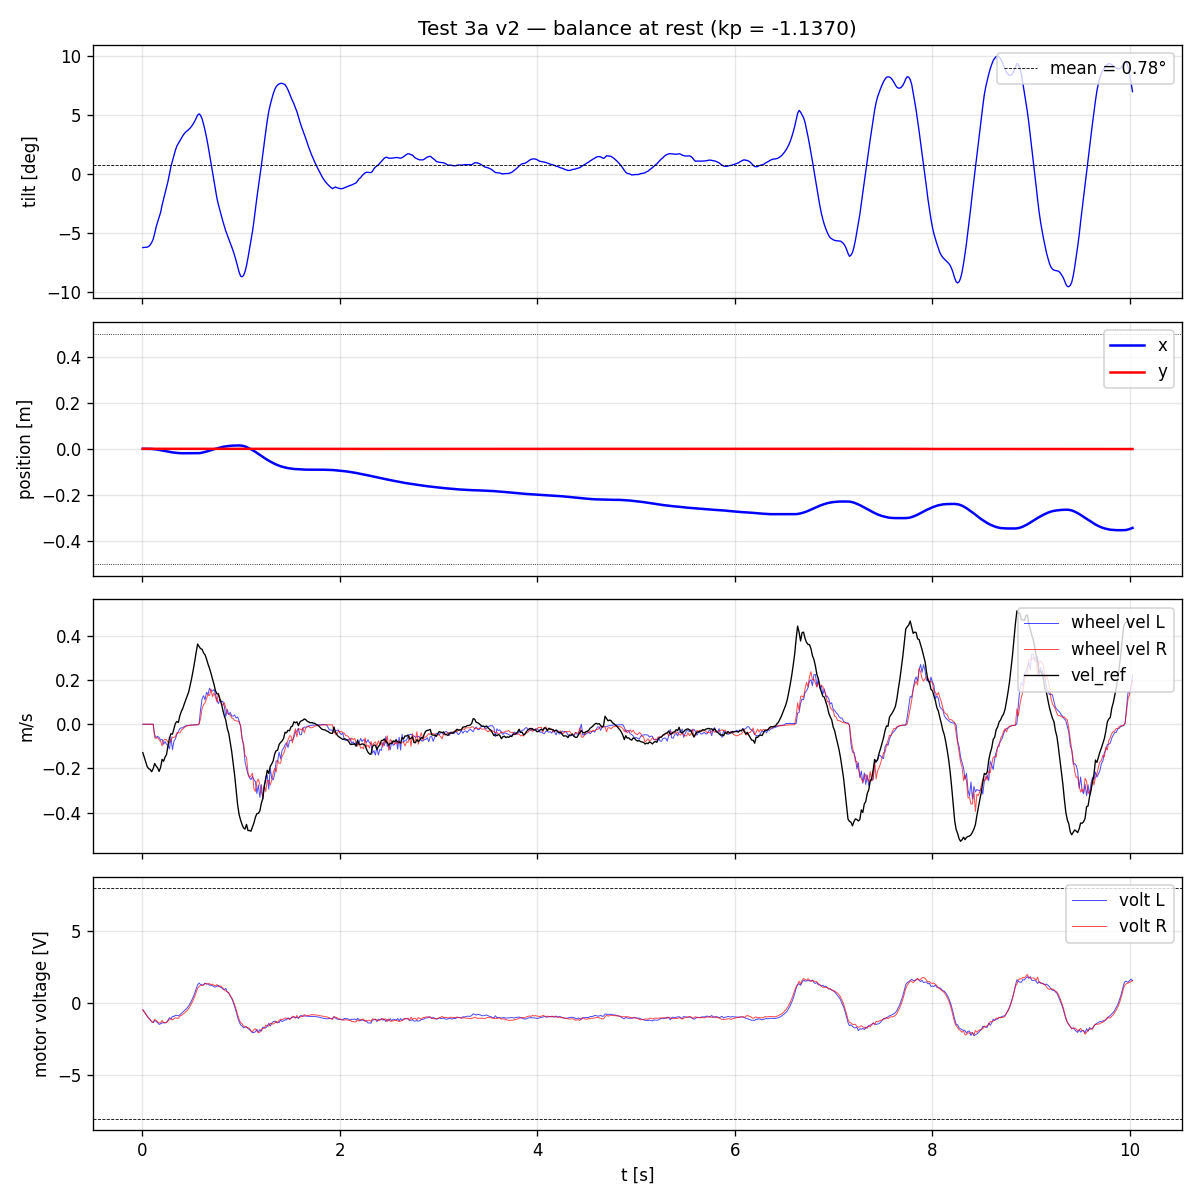
\includegraphics[width=0.85\linewidth]{images/test3a_balance_rest_2026-04-21_v2.png}
    \caption{Task~2 hardware test (Test~3a, v2 run --- reportable for drift specification). From top: tilt angle, linear position, wheel velocity with $\text{vel}_{\text{ref}}$, motor voltages. Balance held for the full 10\,s with $0.343\,\mathrm{m}$ drift and no saturation.}
    \label{fig:task2_hw_3a}
\end{figure}

\paragraph{v3 (Day 5 on-floor) run and the drift/tightness trade.} Test~3a was re-run with the redesigned controller on 2026-04-22. Two consecutive attempts were taken, the second after recalibrating the tilt offset. In both, balance was held for the full 10\,s without falling. Key numbers:
\begin{itemize}
    \item \textbf{Balance tightness improved substantially.} Tilt standard deviation dropped from $4.76^{\circ}$ (v2) to $1.87^{\circ}$ (v3, recalibrated) --- a $61\,\%$ reduction. The late-period pitch excursions visible in the v2 plot are absent in v3: the robot sits much more quietly around its setpoint.
    \item \textbf{Drift, however, increased marginally.} v3 drift was $0.505\,\mathrm{m}$ after recalibration, $0.475\,\mathrm{m}$ before --- either at or slightly above the $0.5\,\mathrm{m}$ spec. The mean tilt offset measured in both v3 runs was $\approx +1.1^{\circ}$, essentially unchanged by the Y-offset recalibration from $176$ to $175$. The static mis-calibration is either one further iteration away from zero or a physical CG/wheel-radius asymmetry that the tilt-offset calibration cannot eliminate. Because the redesigned controller tracks tilt more tightly, this residual $\approx 1^{\circ}$ bias integrates into linear drift more efficiently than the looser v2 controller did.
\end{itemize}
Drift depends on sensor calibration and minor mechanical asymmetries that sit outside the balance controller's authority, whereas tilt tightness directly reflects the controller's authority over the balance loop. For that reason the drift-based specification compliance is evidenced using the v2 run, and the redesign's improvement is reported through the tilt-std reduction. Both results are hardware measurements on the same robot; the difference is which campaign's calibration they were taken under. The v3 Test~3a plot is reproduced in Figure~\ref{fig:task2_hw_3a_v3} for comparison.

\begin{figure}[H]
    \centering
    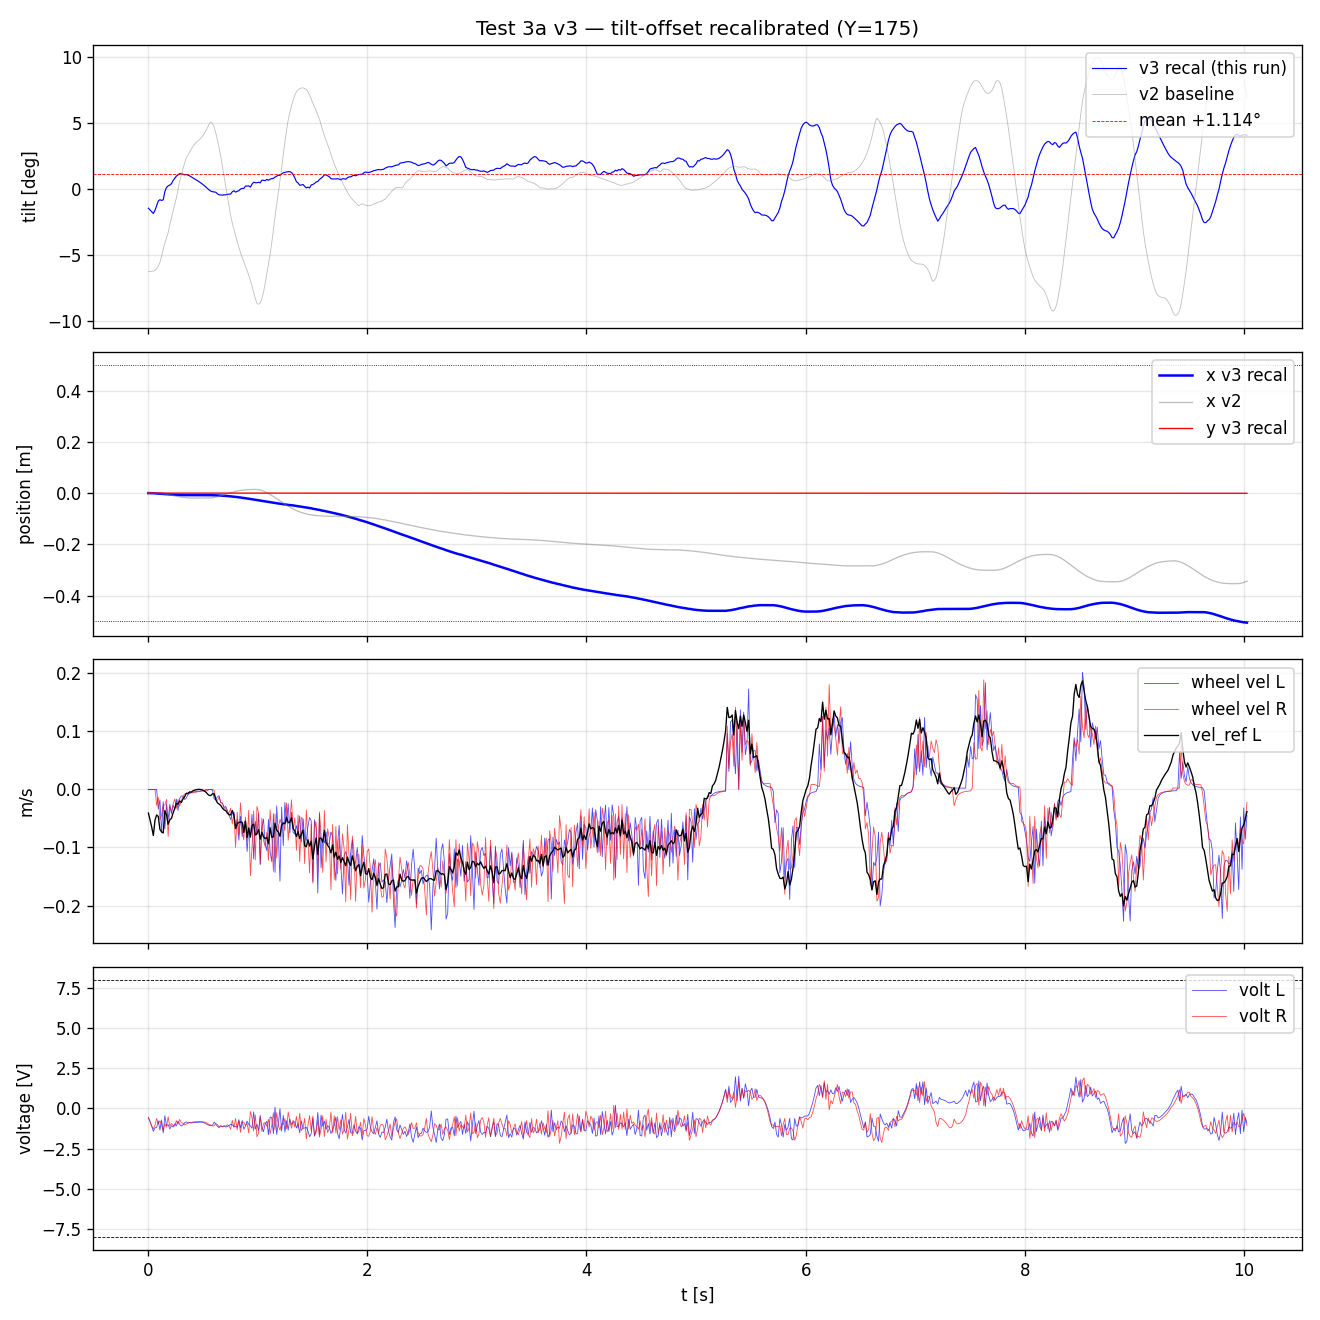
\includegraphics[width=0.85\linewidth]{images/test3a_balance_rest_v3_onfloor_2026-04-22.png}
    \caption{Task~2 hardware test (Test~3a, v3 recalibrated run --- cited for balance tightness). Tilt standard deviation $1.87^{\circ}$ (v2: $4.76^{\circ}$) and the late-period pitch growth visible in Figure~\ref{fig:task2_hw_3a} is absent. Drift is $0.505\,\mathrm{m}$, marginally over spec due to a residual $\approx +1.1^{\circ}$ tilt-offset bias that the tighter v3 controller integrates more cleanly into linear motion.}
    \label{fig:task2_hw_3a_v3}
\end{figure}

\subsection{Comments}
\begin{itemize}
    \item \textbf{Backward drift has two sources.} The mean tilt offset is the dominant one: a residual $\approx 1^{\circ}$ error in the horizontal reference causes the controller to drive the wheels slowly to keep the (mis-measured) tilt at zero. A second, smaller source is any small left/right wheel-radius or drivetrain asymmetry. The on-floor redesign does not change either, so these effects remain the limiting factor for drift --- even as tilt tracking improves.
    \item \textbf{Late-period pitch growth in v2 is largely gone in v3.} In the v2 plot, pitch swings grow from $\pm 5^{\circ}$ at $t \approx 6\,\mathrm{s}$ to $\pm 10^{\circ}$ by $t \approx 10\,\mathrm{s}$, bounded but visible. In the v3 plot the late-period tilt distribution is much flatter, with no corresponding growth. This is an illustrative win from the redesign: the tighter balance loop rejects small environmental perturbations (battery droop, footsteps nearby, floor-slope changes) more aggressively.
\end{itemize}

The sign-flip finding confirms the structure of Lecture~10 Method~2: the minus sign is not cosmetic, it belongs somewhere in the physical loop, and the firmware leaves that choice to the user.
